\section{Conclusions}

This note has discussed the multiple coloumb technique for estimating the energy of a three dimensional reconstructed track, providing motivation for demonstration of the capabilities of this tool within the neutrino LArTPC community. The details of the implementation of this code have been described. The gaussian nature of scatters predicted by the Highland formula has been demonstrated. Additionally the performance of this method has been quantified in two different forms of simulation of fully contained tracks (single muons, and selected BNB neutrino events) as well as in {\ub} data. To summarize the performance on these different fully contained track samples, the bias and resolution for the different samples are overlaid in Figure \ref{MCS_range_bias_resolution_masteroverlay_fig}. Other uses besides energy reconstruction for the MCS technique have been described, including using it as a tool for identification of poorly reconstructed tracks, determination of track direction, particle identification.  XXX this conclusion could definitely be expanded upon.

\begin{figure}
\centering
\mbox{
	\subfigure[\textit{MCS energy bias as a function of range energy.}]
	{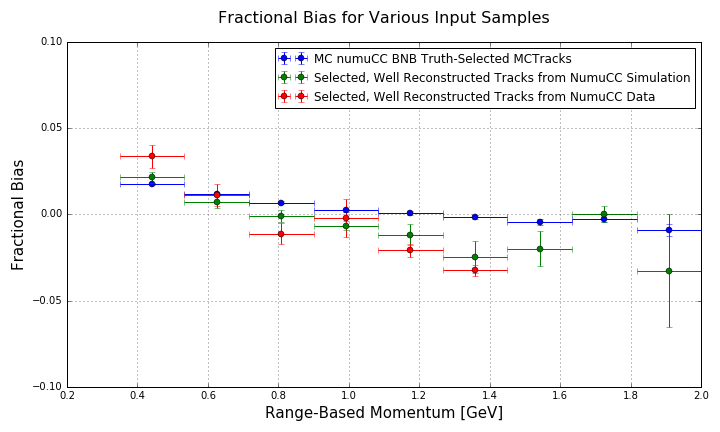
\includegraphics[width=80mm]{Figures/MCS_range_bias_multiplesamples.png}}
	\quad
	\subfigure[\textit{MCS energy resolution as a function of range energy.}]
	{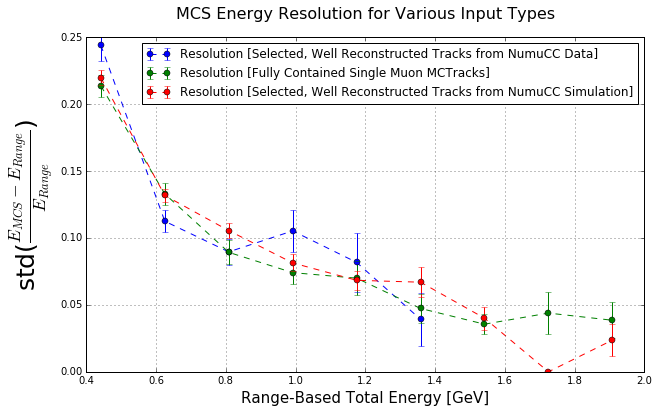
\includegraphics[width=80mm]{Figures/MCS_range_resolution_multiplesamples.png}}
	}
\caption{\textit{MCS energy bias and resolution as a function of range energy for three different input samples: fully contained single muon simulated {\sc MCTracks} discussed in Section \ref{singlemu_mctrack_performance_section} (green), fully contained well reconstructed selected tracks in full BNB simulation discussed in Section \ref{MC_performance_section} (red), and fully contained well reconstructed selected tracks in BNB data discussed in Section \ref{data_performance_section} (blue).}}
\label{MCS_range_bias_resolution_masteroverlay_fig}
\end{figure}
